\documentclass[a4paper,12pt]{article}
\usepackage[left=2cm,right=2cm,top=2cm,bottom=2cm]{geometry}
\usepackage{tikz}

%\title{Ti$k$Z reference}
%\author{Yi-Chen Zhang}
%\date{\today}

\begin{document}
\begin{center}
	\textbf{\Large Ti$k$Z reference}\\
	\bigskip
	Yi-Chen Zhang\\
	\smallskip
	\today
\end{center}

The Ti$k$Z commands can be inside the environment \textbackslash begin\{tikzpicture\} \ldots \textbackslash end\{tikzpicture\} or simply use \textbackslash tikz clause. We run \textsf{pdflatex} or \textsf{latex} followed by \textsf{dvips} to execute the Ti$k$Z commends. 

\section{Straight Path Construction}
%Let's get started with drawing a path. A path is a series of straight lines and curves that are connected. We start a path by specifying the coordinates of the start position as a point in brackets, as in $(0,0)$. The starting point is followed by a series of path extension operators `\textsf{-}\textsf{-}'. Then it must be followed by another coordinate and extends the path in a straight line to a new position. We can put some options in square brackets to describe the properties of the lines. This will be discussed later.
\begin{verbatim}
Useage:
  \draw[options] (x1,y1) -- (x2,y2) -- (x3,y3);

Example:
  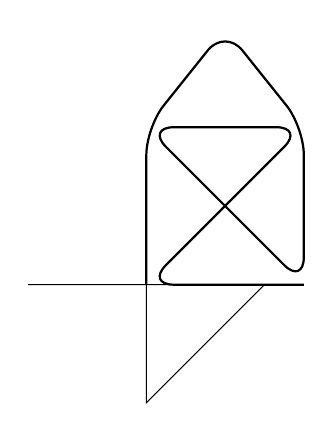
\begin{tikzpicture}
    \draw (-1.5,0) -- (1.5,0) -- (0,-1.5) -- (0,1.5);
    \draw[thick, rounded corners=10pt] (0,0) -- (0,2) -- (1,3.25) -- 
      (2,2) -- (2,0) -- (0,2) -- (2,2) -- (0,0) -- (2,0);
  \end{tikzpicture}
\end{verbatim}

\tikz \draw (-1.5,0) -- (1.5,0) -- (0,-1.5) -- (0,1.5);
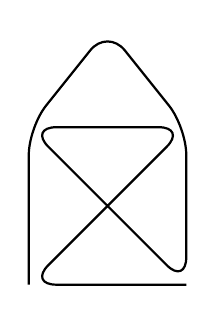
\begin{tikzpicture}
  \draw[thick, rounded corners=10pt] (0,0) -- (0,2) -- (1,3.25) -- (2,2) -- (2,0) -- (0,2) -- (2,2) -- (0,0) -- (2,0); % -- cycle;
\end{tikzpicture}

\section{Circle Path Construction}
\begin{verbatim}
Usage:
  \draw[options] (x,y) circle (raidus);
  \draw[options] (x,y) ellipse (x.raidus anda y.radius);

Example:
  
\begin{tikzpicture}
    \draw (0,0) circle (2pt);
    \draw[red] (1,0) circle (3pt);
    \draw[fill=red] (2,0) circle (4pt);
    \draw[red,fill=red] (3,0) ellipse (10pt and 5pt);
    \filldraw[blue,rotate=30] (3.5,-2) ellipse (10pt and 5pt); % another way
  \end{tikzpicture}
\end{verbatim}


\begin{tikzpicture}
  \draw (0,0) circle (2pt);
  \draw[red] (1,0) circle (3pt);
  \draw[fill=red] (2,0) circle (4pt);
  \draw[red,fill=red] (3,0) ellipse (10pt and 5pt);
  \filldraw[blue,rotate=30] (3.5,-2) ellipse (10pt and 5pt);
\end{tikzpicture}

\section{Curved Path Construction}
\begin{verbatim}
Usage:
  \draw[options] (x1,y1) .. controls (x2,y2) and (x3,y3) .. (x4,y4);

Example:
  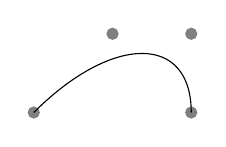
\begin{tikzpicture}
    \filldraw[gray] (0,0) circle (2pt) (1,1) circle (2pt)
                    (2,1) circle (2pt) (2,0) circle (2pt);
    \draw (0,0) .. controls (1,1) and (2,1) .. (2,0);
  \end{tikzpicture}
\end{verbatim}

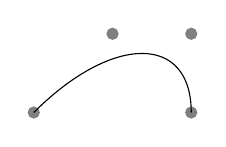
\begin{tikzpicture}
  \filldraw[gray] (0,0) circle (2pt) (1,1) circle (2pt)
                  (2,1) circle (2pt) (2,0) circle (2pt);
  \draw (0,0) .. controls (1,1) and (2,1) .. (2,0);
\end{tikzpicture}

\section{Rectangle Path Construction}
\begin{verbatim}
Usage:
  \draw[options] (x1,y1) rectangle (x2,y2);
  \draw[options] (x,y) rectangle +(width,height);

Example:
  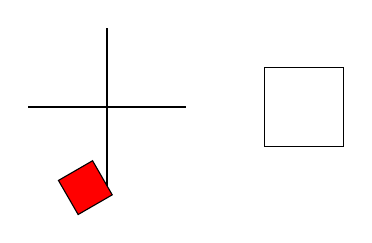
\begin{tikzpicture}
    \draw (-1,0) -- (1,0);
    \draw (0,-1) -- (0,1);
    \draw[rotate=30, fill=red] (-0.5,-0.5) rectangle (-1,-1);
    \draw (2,-0.5) rectangle +(1,1);
  \end{tikzpicture}
\end{verbatim}

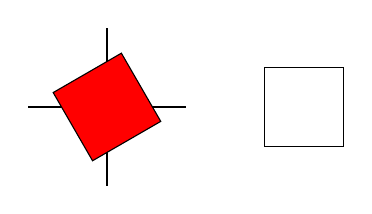
\begin{tikzpicture}
  \draw (-1,0) -- (1,0);
  \draw (0,-1) -- (0,1);
  \draw[rotate=30, fill=red] (-0.5,-0.5) rectangle (0.5,0.5);
	\draw (2,-0.5) rectangle +(1,1);
\end{tikzpicture}

\section{Grid Path Construction}
\begin{verbatim}
Usage:
  \draw[options] (x1,y1) grid (x2,y2); 
\end{verbatim}

\begin{verbatim}
Example:
  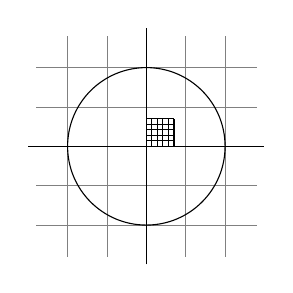
\begin{tikzpicture}
    \draw[step=.5cm, gray, very thin] (-1.4,-1.4) grid (1.4,1.4);
    \draw (-1.5,0) -- (1.5,0);
    \draw (0,-1.5) -- (0,1.5);
    \draw (0,0) circle (1cm);
    \draw[step=2pt] (0,0) grid (10pt,10pt);
  \end{tikzpicture}
\end{verbatim}

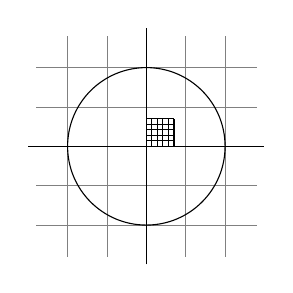
\begin{tikzpicture}
	\draw[step=.5cm, gray, very thin] (-1.4,-1.4) grid (1.4,1.4);
	\draw (-1.5,0) -- (1.5,0);
	\draw (0,-1.5) -- (0,1.5);
	\draw (0,0) circle (1cm);
  \draw[step=2pt] (0,0) grid (10pt,10pt);
\end{tikzpicture}

\section{Drawing Options}
There are some drawing options that one can use to control the color, thickness, and line type.
\begin{itemize}
  \item color: 
    blue \tikz \filldraw[blue] (0,0) rectangle (1.5em,1.5ex);, 
    black \tikz \filldraw[black] (0,0) rectangle (1.5em,1.5ex);, 
    brown \tikz \filldraw[brown] (0,0) rectangle (1.5em,1.5ex);, 
    cyan \tikz \filldraw[cyan] (0,0) rectangle (1.5em,1.5ex);, 
    gray \tikz \filldraw[gray] (0,0) rectangle (1.5em,1.5ex);, 
    green \tikz \filldraw[green] (0,0) rectangle (1.5em,1.5ex);, 
    lightgray \tikz \filldraw[lightgray] (0,0) rectangle (1.5em,1.5ex);, 
    lime \tikz \filldraw[lime] (0,0) rectangle (1.5em,1.5ex);, 
    magenta \tikz \filldraw[magenta] (0,0) rectangle (1.5em,1.5ex);, 
    orange \tikz \filldraw[orange] (0,0) rectangle (1.5em,1.5ex);, 
    pink \tikz \filldraw[pink] (0,0) rectangle (1.5em,1.5ex);, 
    purple \tikz \filldraw[purple] (0,0) rectangle (1.5em,1.5ex);, 
    red \tikz \filldraw[red] (0,0) rectangle (1.5em,1.5ex);, 
    yellow \tikz \filldraw[yellow] (0,0) rectangle (1.5em,1.5ex);, 
    teal \tikz \filldraw[teal] (0,0) rectangle (1.5em,1.5ex);, 
    violet \tikz \filldraw[violet] (0,0) rectangle (1.5em,1.5ex);, 
    white \tikz \draw[fill=white] (0,0) rectangle (1.5em,1.5ex);.\\
    Note: Colors can also be mixed. The color \verb|[blue!40!white]| means $40\%$ blue and $60\%$ white mixed together.
  \item thickness: 
    ultra thin \begin{tikzpicture} \filldraw[white] (0,0) rectangle (1em,1.5ex); \draw[ultra thin] (0,0.7ex) -- (1em,0.7ex);\end{tikzpicture}, 
    very thin \begin{tikzpicture} \filldraw[white] (0,0) rectangle (1em,1.5ex); \draw[very thin] (0,0.7ex) -- (1em,0.7ex);\end{tikzpicture}, 
    thin \begin{tikzpicture} \filldraw[white] (0,0) rectangle (1em,1.5ex); \draw[thin] (0,0.7ex) -- (1em,0.7ex);\end{tikzpicture}, 
    semithick \begin{tikzpicture} \filldraw[white] (0,0) rectangle (1em,1.5ex); \draw[semithick] (0,0.7ex) -- (1em,0.7ex);\end{tikzpicture}, 
    thick \begin{tikzpicture} \filldraw[white] (0,0) rectangle (1em,1.5ex); \draw[thick] (0,0.7ex) -- (1em,0.7ex);\end{tikzpicture}, 
    very thick \begin{tikzpicture} \filldraw[white] (0,0) rectangle (1em,1.5ex); \draw[very thick] (0,0.7ex) -- (1em,0.7ex);\end{tikzpicture}, 
    ultra thick \begin{tikzpicture} \filldraw[white] (0,0) rectangle (1em,1.5ex); \draw[ultra thick] (0,0.7ex) -- (1em,0.7ex);\end{tikzpicture}.\\
    Note: \verb![help lines]=[gray,very thin]!. Line thickness can be also specified by\\ \verb![line width]! option, say \verb![line width=0.5cm]!.
  \item line type: 
    loosely dashed \begin{tikzpicture} \filldraw[white] (0,0) rectangle (1em,1.5ex); \draw[loosely dashed] (0,0.7ex) -- (1em,0.7ex);\end{tikzpicture},
    dashed \begin{tikzpicture} \filldraw[white] (0,0) rectangle (1em,1.5ex); \draw[dashed] (0,0.7ex) -- (1em,0.7ex);\end{tikzpicture},
    densely dashed \begin{tikzpicture} \filldraw[white] (0,0) rectangle (1em,1.5ex); \draw[densely dashed] (0,0.7ex) -- (1em,0.7ex);\end{tikzpicture},
    loosely dotted \begin{tikzpicture} \filldraw[white] (0,0) rectangle (1em,1.5ex); \draw[loosely dotted] (0,0.7ex) -- (1em,0.7ex);\end{tikzpicture},
    dotted \begin{tikzpicture} \filldraw[white] (0,0) rectangle (1em,1.5ex); \draw[dotted] (0,0.7ex) -- (1em,0.7ex);\end{tikzpicture},
    densely dotted \begin{tikzpicture} \filldraw[white] (0,0) rectangle (1em,1.5ex); \draw[densely dotted] (0,0.7ex) -- (1em,0.7ex);\end{tikzpicture}.
  \item arrow: 
    \verb!<-! \begin{tikzpicture} \filldraw[white] (0,0) rectangle (1em,1.5ex); \draw[<-] (0,0.7ex) -- (1em,0.7ex);\end{tikzpicture},
    \verb!<<-! \begin{tikzpicture} \filldraw[white] (0,0) rectangle (1em,1.5ex); \draw[<<-] (0,0.7ex) -- (1em,0.7ex);\end{tikzpicture},
    \verb!<-|! \begin{tikzpicture} \filldraw[white] (0,0) rectangle (1em,1.5ex); \draw[<-|] (0,0.7ex) -- (1em,0.7ex);\end{tikzpicture},
    \verb!<<-|! \begin{tikzpicture} \filldraw[white] (0,0) rectangle (1em,1.5ex); \draw[<<-|] (0,0.7ex) -- (1em,0.7ex);\end{tikzpicture},
    \verb!->! \begin{tikzpicture} \filldraw[white] (0,0) rectangle (1em,1.5ex); \draw[->] (0,0.7ex) -- (1em,0.7ex);\end{tikzpicture},
    \verb!->>! \begin{tikzpicture} \filldraw[white] (0,0) rectangle (1em,1.5ex); \draw[->>] (0,0.7ex) -- (1em,0.7ex);\end{tikzpicture},
    \verb!|->! \begin{tikzpicture} \filldraw[white] (0,0) rectangle (1em,1.5ex); \draw[|->] (0,0.7ex) -- (1em,0.7ex);\end{tikzpicture},
    \verb!|->>! \begin{tikzpicture} \filldraw[white] (0,0) rectangle (1em,1.5ex); \draw[|->>] (0,0.7ex) -- (1em,0.7ex);\end{tikzpicture},
    \verb!<->! \begin{tikzpicture} \filldraw[white] (0,0) rectangle (1em,1.5ex); \draw[<->] (0,0.7ex) -- (1em,0.7ex);\end{tikzpicture},
    \verb!<<->>! 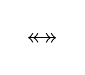
\begin{tikzpicture} \filldraw[white] (0,0) rectangle (1em,1.5ex); \draw[<<->>] (0,0.7ex) -- (1em,0.7ex);\end{tikzpicture}.\\
    Note: You can also add \verb!>=stealth! in the options, which changes the arrow to 'stealth-like' style.
\end{itemize}

\begin{verbatim}
Usage:
  \draw[color, thickness, line type, arrow] (x1,y1) -- (x2,y2);

Example:
  
\begin{tikzpicture}
    \draw[red, very thin, densely dashed, <-] (0,0) -- (0.9,0);
    \draw[green, ultra thick, loosely dotted, |->] (1.1,0) -- (1.9,0);
    \draw[blue, semithick, <->, >=stealth] (2.1,0) -- (2.9,0);
    \draw[purple, line width=0.3cm] (3.1,0) -- (3.9,0);
  \end{tikzpicture}
\end{verbatim}


\begin{tikzpicture}
  \draw[red, very thin, densely dashed, <-] (0,0) -- (0.9,0);
  \draw[green, ultra thick, loosely dotted, |->] (1.1,0) -- (1.9,0);
  \draw[blue, semithick, <->, >=stealth] (2.1,0) -- (2.9,0);
  \draw[purple, line width=0.3cm] (3.1,0) -- (3.9,0);
\end{tikzpicture}

\section{Arc Path Construction}
\begin{verbatim}
Usage:
  \draw (x,y) arc (angle1:angle2:radius);
  \draw (x,y) arc [start angle=angle1, end angle=angle2, radius=radius];
  \draw (x,y) arc (angle1:angle2:x.radius and y.radius);
  \draw (x,y) arc [start angle=angle1, end angle=angle2, x radius=rx, y radius=ry]

Example:
  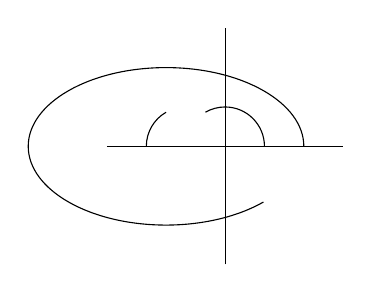
\begin{tikzpicture}
    \draw (-1.5,0) -- (1.5,0);
    \draw (0,-1.5) -- (0,1.5);
    \draw (0.5,0) arc (0:120:0.5cm);
    \draw (1,0) arc (0:315:1.75cm and 1cm);
    \draw (-1,0) arc [start angle=180, end angle=120, radius=0.5cm];
    % The above is not a recommand way.
  \end{tikzpicture}
\end{verbatim}

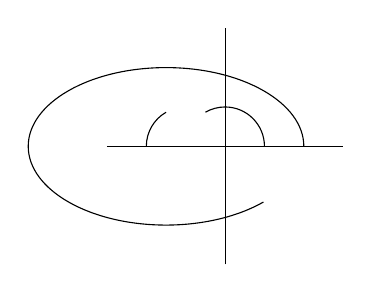
\begin{tikzpicture}
  \draw (-1.5,0) -- (1.5,0);
  \draw (0,-1.5) -- (0,1.5);
  \draw (0.5,0) arc (0:120:0.5cm);
  \draw (1,0) arc (0:315:1.75cm and 1cm);
  \draw (-1,0) arc [start angle=180, end angle=120, radius=0.5cm];
\end{tikzpicture}

\section{Adding a Touch Style}
\noindent 
\textsf{Styles} are predefined sets of options that can be used to organize how a graphic is drawn. To define a style globally, we can use the \textbackslash tikzset command at the beginning of the document.
\begin{verbatim}
Usage:
  \tikzset{style_name./style={options}}

Example:
  \tikzset{blue_thin_lines/.style={color=blue!50,very thin}}
  \begin{tikzpicture}
    \draw[blue_thin_lines] (0,0) grid (5,5);
  \end{tikzpicture}
\end{verbatim}

\tikzset{blue_thin_lines/.style={color=blue!50,very thin}}
\begin{tikzpicture}
	\draw[step=0.5cm, blue_thin_lines] (0,0) grid (2,2);
\end{tikzpicture}\\

\noindent To define a style locally, we use a pair of square bracket ``[ ]'' to define styles at the beginning of a picture.
\begin{verbatim}
Usage:
  [style_name/.style={options}]

Example:
  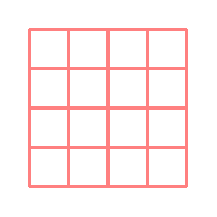
\begin{tikzpicture}
    [red_thick_lines/.style={color=red!50,very thick}];
    \draw[step=0.5cm, red_thick_lines] (0,0) grid (2,2);
  \end{tikzpicture}
\end{verbatim}

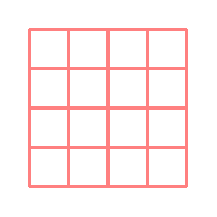
\begin{tikzpicture}
	[red_thick_lines/.style={color=red!50,very thick}]
	\draw[step=0.5cm, red_thick_lines] (0,0) grid (2,2);
\end{tikzpicture}\\

\noindent One can also define styles hierarchically.
\begin{verbatim}
Usage:
  \tikzset{style_name1/.style={style_name2, options}}

Example:
  \tikzset{green_help_lines/.style={help lines, color=green!90}}
  \begin{tikzpicture}
    \draw[step=0.5cm, green_help_lines] (0,0) grid (5,5);
  \end{tikzpicture}
\end{verbatim}

\tikzset{green_help_lines/.style={help lines, color=green!90, ultra thick}}
\begin{tikzpicture}
  \draw[step=0.5cm, help lines] (0,0) grid (2,2);
  \draw[step=0.5cm, green_help_lines] (2,0) grid (4,2);
\end{tikzpicture}\\

\noindent Styles can also be used with a parameter.
\begin{verbatim}
Usage:
  [style_name/.style={options}, style_name/.default={options}]

Example:
  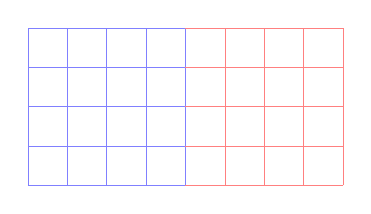
\begin{tikzpicture}
    [para_color/.style={help lines,color=#1!50}, para_color/.default=blue]
    \draw[step=0.5cm, para_color] (0,0) grid (2,2);
    \draw[step=0.5cm, para_color=red] (2,0) grid (4,2);
  \end{tikzpicture}
\end{verbatim}

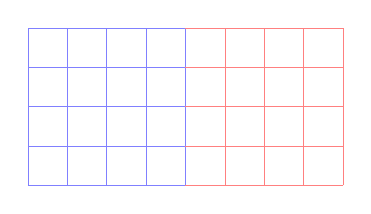
\begin{tikzpicture}
  [para_color/.style={help lines,color=#1!50}, para_color/.default=blue]
  \draw[step=0.5cm, para_color] (0,0) grid (2,2);
  \draw[step=0.5cm, para_color=red] (2,0) grid (4,2);
\end{tikzpicture}

\section{Clipping a Path}
\noindent The \textbackslash clip command clip all subsequent drawing.
\begin{verbatim}
Usage:
  \clip[options] (x1,y1) rectangle (x2,y2);

Example:
  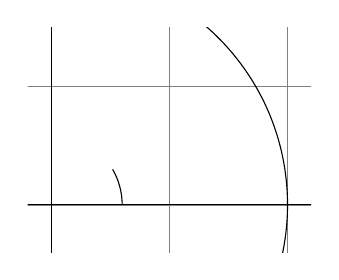
\begin{tikzpicture}[scale=3]
    \clip (-0.1,-0.2) rectangle (1.1,0.75);
    \draw[step=.5cm, help lines] (-1.4,-1.4) grid (1.4,1.4);
    \draw (-1.5,0) -- (1.5,0);
    \draw (0,-1.5) -- (0,1.5);
    \draw (0,0) circle (1cm);
    \draw (3mm,0mm) arc (0:30:3mm);
  \end{tikzpicture}
\end{verbatim}

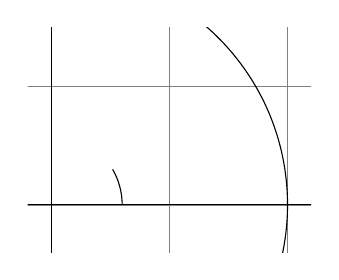
\begin{tikzpicture}[scale=3]
	\clip (-0.1,-0.2) rectangle (1.1,0.75);
	\draw[step=.5cm, help lines] (-1.4,-1.4) grid (1.4,1.4);
	\draw (-1.5,0) -- (1.5,0);
	\draw (0,-1.5) -- (0,1.5);
	\draw (0,0) circle (1cm);
	\draw (3mm,0mm) arc (0:30:3mm);
\end{tikzpicture}

\begin{verbatim}
Usage:
  \clip (x1,y1) circle (radius);

Example:
  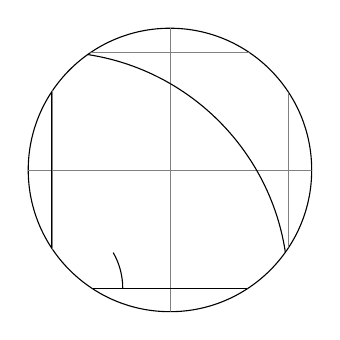
\begin{tikzpicture}[scale=3]
    \clip[draw] (0.5,0.5) circle (.6cm);
    \draw[step=.5cm, help lines] (-1.4,-1.4) grid (1.4,1.4);
    \draw (-1.5,0) -- (1.5,0);
    \draw (0,-1.5) -- (0,1.5);
    \draw (0,0) circle (1cm);
    \draw (3mm,0mm) arc (0:30:3mm);
  \end{tikzpicture}
\end{verbatim}

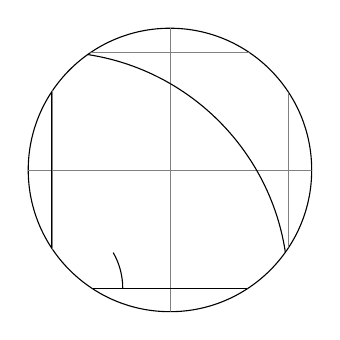
\begin{tikzpicture}[scale=3]
  \clip[draw] (0.5,0.5) circle (.6cm);
  \draw[step=.5cm, help lines] (-1.4,-1.4) grid (1.4,1.4);
  \draw (-1.5,0) -- (1.5,0);
  \draw (0,-1.5) -- (0,1.5);
  \draw (0,0) circle (1cm);
  \draw (3mm,0mm) arc (0:30:3mm);
\end{tikzpicture}

\section{Parabola Path Construction}
\begin{verbatim}
Usage:
  \draw[options] (x1,y1) parabola (x2,y2);

Example:
  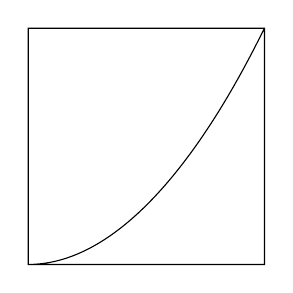
\begin{tikzpicture}[scale=3]
    \draw (0,0) rectangle (1,1) (0,0) parabola (1,1);
  \end{tikzpicture}
\end{verbatim}

\begin{tikzpicture}
  \draw (0,0) rectangle (2,2) (0,0) parabola (2,2);
\end{tikzpicture}

\begin{verbatim}
Usage:
  \draw[options] (x1,y1) parabola bend (x2,y2) (x3,y3);

Example:
  \begin{tikzpicture}
    \draw[x=0.2cm,y=0.2cm] (0,0) parabola bend (4,10) (6,6);
  \end{tikzpicture}
\end{verbatim}

\begin{tikzpicture}
  \draw[x=0.2cm,y=0.2cm] (0,0) parabola bend (4,10) (6,6);
\end{tikzpicture}

\section{Sine and Cosine Path Construction} 
\begin{verbatim}
Usage:
  \draw[options] (x1,y1) sin (x2,y2);
  \draw[options] (x1,y1) cos (x2,y2);

Example:
  \begin{tikzpicture}
    \draw[help lines] (-0.5,-1.5) grid (4.5,1.5);
    \draw[red] (0,0) sin (1,1) cos (2,0) sin (3,-1) cos (4,0);
    \draw[blue] (0,1) cos (1,0) sin (2,-1) cos (3,0) sin (4,1);
  \end{tikzpicture}
\end{verbatim}

\begin{tikzpicture}
  \draw[help lines] (-0.5,-1.5) grid (4.5,1.5);
  \draw[red] (0,0) sin (1,1) cos (2,0) sin (3,-1) cos (4,0);
  \draw[blue] (0,1) cos (1,0) sin (2,-1) cos (3,0) sin (4,1);
\end{tikzpicture}

\section{Filling and Drawing}
\begin{verbatim}
Usage:
  \fill[options] (x1,y1) -- (x2,y2) arc (angle1:angle2:radius) -- (x3,y3);
  \fill[options] (x1,y1) -- (x2,y2) arc (angle1:angle2:radius) -- cycle; % better
  \filldraw[options] (x1,y1) -- (x2,y2) arc (angle1:angle2:radius) -- cycle;

Example:
  \begin{tikzpicture}[line width=5pt]
    \fill[blue!80] (0,0) -- (3,0) arc (0:30:2) -- (0,0);
    \draw (4,0) -- (5,0) -- (5,1) -- (4,0);
    \draw (6,0) -- (7,0) -- (7,1) -- cycle;
    \filldraw[fill=green!20!white, draw=green!50!black]
      (8,0) -- (11,0) arc (0:45:3) -- cycle;
  \end{tikzpicture}
\end{verbatim}

\begin{tikzpicture}[line width=5pt]
  \fill[blue!80] (0,0) -- (3,0) arc (0:30:2) -- (0,0);
  \draw (4,0) -- (5,0) -- (5,1) -- (4,0);
  \draw (6,0) -- (7,0) -- (7,1) -- cycle;
  \filldraw[fill=green!20!white, draw=green!50!black]
    (8,0) -- (11,0) arc (0:45:3) -- cycle;
\end{tikzpicture}

\section{Shading}
\begin{verbatim}
Usage:
  \shade[options] (x1,y1) rectangle (x2,y2);
  \shadedraw[options] (x1,y1) circle (radius);

Example:
  \begin{tikzpicture}[rounded corners,ultra thick]
    \shade (0,0) rectangle (2,1);
    \shadedraw (3,0.5) circle (.5cm);
    \shade[top color=yellow,bottom color=black] (0,0) rectangle +(2,1);
    \shade[left color=yellow,right color=black] (3,0) rectangle +(2,1);
    \shadedraw[inner color=yellow,outer color=black,draw=yellow] 
      (6,0) rectangle +(2,1);
    \shade[ball color=green] (9,.5) circle (.5cm);
    \shadedraw[left color=gray,right color=green, draw=green!50!black]
      (10,0.3) -- +(1,0) arc (0:30:1) -- cycle;
  \end{tikzpicture}
\end{verbatim}

\begin{tikzpicture}[rounded corners,ultra thick]
  \shade (0,0) rectangle (2,1);
  \shadedraw (3,0.5) circle (.5cm);
  \shade[top color=yellow,bottom color=black] (4,0) rectangle +(2,1);
  \shade[left color=yellow,right color=black] (7,0) rectangle +(2,1);
  \shadedraw[inner color=yellow,outer color=black,draw=yellow] (10,0) rectangle +(2,1);
  \shade[ball color=green] (13,.5) circle (.5cm);
  \shadedraw[left color=gray,right color=green, draw=green!50!black]
    (14,0.3) -- +(1,0) arc (0:30:1) -- cycle;
\end{tikzpicture}

\section{Specifying Coordinates}
\begin{verbatim}
Usage:
  (xpt,ycm): xpt in x-direction and ycm in y-directions.
  (xdegree:ycm): ycm in direction x degree.
  +(x,y): xcm above and ycm right from the previous specified position.
  ++(x,y): xcm above and ycm right from the previous specified position 
           and making this the new specified position.
  (x1,y1) -- (x2,y2): straight line from (x1,y1) to (x2,y2);
  (x1,y1) -| (x2,y2): a horizontal and vertical line from (x1,y1) to (x2,y2);
  (x1,y1) |- (x2,y2); a vertical and horizontal line from (x1,y1) to (x2,y2);

Example:
  \begin{tikzpicture}
    \draw[red,very thick] (30:1cm) -- (0,0);
    \draw[blue,very thick] (0,0) -| +(1.5,0.5) ;
    \draw[green,very thick] (0,0) |- ++(0,1) -- (1,0);
  \end{tikzpicture}
\end{verbatim}

\begin{tikzpicture}
  \draw[red,very thick] (30:1cm) -- (0,0);
  \draw[blue,very thick] (0,0) -| +(1.5,0.5) ;
  \draw[green,very thick] (0,0) ++(0,1) -- (1,0);
\end{tikzpicture}

\section{Scoping}
\begin{verbatim}
Usage:
  \begin{scope}[options]
    % only apply graphic options inside this scope, but not to anything outside.
  \end{scope}

Example:
  \begin{tikzpicture}[ultra thick]
    \draw (0,0) -- (0,1);
    \begin{scope}[thin]
      \draw (1,0) -- (1,1);
    \end{scope}
    \draw (2,0) -- (2,1);
  \end{tikzpicture}
\end{verbatim}

\begin{tikzpicture}[ultra thick]
  \draw (0,0) -- (0,1);
	\begin{scope}[thin]
		\draw (1,0) -- (1,1);
	\end{scope}
	\draw (2,0) -- (2,1);
\end{tikzpicture}

\section{Transformations}
\begin{verbatim}
Usage:
  [xshift=x,yshift=y]: allows you to shift all subsequent points by x and y amount.
  [shift={(x,y)}] or [shift={+(x,y)}];

  [rotate=angle]: rotating by a certain angle.
  [rotate around={angle:(x,y)}]: rotating around a given point by a certain angle.

  [xscale=unit1,yscale=unit2]: scaling the x-direction or y-direction.
  [scale=unit]: scaling by a certain factor

  [xslant=unit1,yslant=unit2]: slanting the x-direction or y-direction. 

Example:
  \begin{tikzpicture}
    \draw[help lines, step=0.5] (0,0) grid (7,1.5);
    \draw[red, very thick] (0,0) -- (0,0.5) 
         [shift={(4pt,2pt)}] (0,0) -- (0,0.5);
    \draw[red, very thick] (0.5,0) -- (0.5,0.5) 
         [shift={+(4pt,2pt)}] (0.5,0) -- (0.5,0.5);
    \draw[rotate=30,fill=blue] (1.5,-1) rectangle (2,-0.5);
    \draw[rotate around={60:(3,0.5)},fill=blue] (2.5,0.25) rectangle (3,0.75);
    \draw[xscale=1,yscale=1.1,fill=green] (4,0.5) circle (0.5);
    \draw[xslant=2,very thick] (5,0) -- (5.5,0.5) -- (5.5,0);
  \end{tikzpicture}
\end{verbatim}

\begin{tikzpicture}
	\draw[help lines, step=0.5] (0,0) grid (7,1.5);
	\draw[red, very thick] (0,0) -- (0,0.5) 
			 [shift={(4pt,2pt)}] (0,0) -- (0,0.5);
	\draw[red, very thick] (0.5,0) -- (0.5,0.5) 
			 [shift={+(4pt,2pt)}] (0.5,0) -- (0.5,0.5);
	\draw[rotate=30,fill=blue] (1.5,-1) rectangle (2,-0.5);
 	\draw[rotate around={60:(3,0.5)},fill=blue] (2.5,0.25) rectangle (3,0.75);
	\draw[xscale=1,yscale=1.1,fill=green] (4,0.5) circle (0.5);
	\draw[xslant=2,very thick] (5,0) -- (5.5,0.5) -- (5.5,0);
\end{tikzpicture}

\begin{verbatim}
  \begin{tikzpicture}
    \filldraw[fill=red] (0,0) rectangle (1,1)
    [xshift=5pt,yshift=5pt] (0,0) rectangle (1,1)
    [rotate=30] (-1,-1) rectangle (2,2);
  \end{tikzpicture}
\end{verbatim}

\begin{tikzpicture}[even odd rule,rounded corners=2pt,x=10pt,y=10pt]
	\filldraw[fill=red] (0,0) rectangle (1,1)
	[xshift=5pt,yshift=5pt] (0,0) rectangle (1,1)
	[rotate=30] (-1,-1) rectangle (2,2);
\end{tikzpicture}

\section{For-Loops}
\begin{verbatim}
Usage:
  \foreach \variable in {list of values}{
    \commands ;
  }
Example:
  \begin{tikzpicture}
    \foreach \x in {-0.5cm,0cm,0.5cm}{
      \draw[red,very thick] (\x,-5pt) -- (\x,5pt);
    }
    \foreach \y in {-0.5cm,0cm,0.5cm}{
      \draw[blue,very thick] (1cm,\y) -- (1.5cm,\y);
    }
    \foreach \x in {0,...,9}{
      \draw[green,very thick] (\x,-1) circle (0.4cm);
    }
    \foreach \x in {2,2.5,...,4}{
      \draw[purple,very thick] (\x cm,-3pt) -- (\x cm,3pt);
    }
  \end{tikzpicture}
\end{verbatim}

\begin{tikzpicture}
  \foreach \x in {-0.5cm,0cm,0.5cm}{
    \draw[red,very thick] (\x,-5pt) -- (\x,5pt);
  }
  \foreach \y in {-0.5cm,0cm,0.5cm}{
    \draw[blue,very thick] (1cm,\y) -- (1.5cm,\y);
  }
  \foreach \x in {0,...,9}{
    \draw[green,very thick] (\x,-1) circle (0.4cm);
  }
  \foreach \x in {2,2.5,...,4}{
    \draw[purple,very thick] (\x cm,-3pt) -- (\x cm,3pt);
  }
\end{tikzpicture}

\begin{verbatim}
  \begin{tikzpicture}
    \foreach \x in {1,2,...,5,7,8,...,12}{
      \foreach \y in {1,...,5}{
        \draw (\x,\y) +(-0.5,-0.5) rectangle +(0.5,0.5);
        \draw (\x,\y) node{\x,\y};
      }
    }
  \end{tikzpicture}
\end{verbatim}

\begin{tikzpicture}
  \foreach \x in {1,2,...,5,7,8,...,12}{
		\foreach \y in {1,...,5}{
			\draw (\x,\y) +(-0.5,-0.5) rectangle +(0.5,0.5);
			\draw (\x,\y) node{\x,\y};
		}
	}
\end{tikzpicture}

% \begin{tikzpicture}
%   \foreach \x in {-1cm,-0.5cm,1cm}

%   \foreach \x in {1,2,3} {$x=\x, $}
% \end{tikzpicture}

\section{Adding Text}
\begin{verbatim}
Usage:
  \draw (x,y) node[options] {text};
  \draw (x,y) node[options] {text};
  \node[options] at (x,y) {text};
  options: above,below,left,right, or anchor=north,south,west,east.

Example:
  \begin{tikzpicture}[scale=2]
    \draw[<->] (0,1) -- (0,0) -- (1,0);
    \draw[fill] (0.5,0.5) circle (0.05);
    \draw (0.5,0.5) node[above=10pt] {A} node[left=10pt] {L} 
                    node[below=10pt] {B} node[right=10pt] {R};
    \draw (0.5,0.5) node[above left=2pt] {AL} node[below left=2pt] {BL} 
                    node[below right=2pt] {BR} node[above right=2pt] {AR};
  \end{tikzpicture}
  \begin{tikzpicture}[scale=2]
    \draw[<->] (0,1) -- (0,0) -- (1,0);
    \draw[fill] (0.5,0.5) circle (0.05);
    \draw (0.5,0.5) node[anchor=north] {N} node[anchor=west] {W} 
                    node[anchor=south] {S} node[anchor=east] {E};
    \draw (0.5,0.5) node[anchor=north west] {NW} node[anchor=south west] {SW} 
                    node[anchor=south east] {SE} node[anchor=north east] {NE};
\end{tikzpicture}
\end{verbatim}

\begin{tikzpicture}[scale=2]
  \draw[<->] (0,1) -- (0,0) -- (1,0);
  \draw[fill] (0.5,0.5) circle (0.05);
  \draw (0.5,0.5) node[above=10pt] {A} node[left=10pt] {L} node[below=10pt] {B} node[right=10pt] {R};
  \draw (0.5,0.5) node[above left=2pt] {AL} node[below left=2pt] {BL} node[below right=2pt] {BR} node[above right=2pt] {AR};
\end{tikzpicture}
\begin{tikzpicture}[scale=2]
  \draw[<->] (0,1) -- (0,0) -- (1,0);
  \draw[fill] (0.5,0.5) circle (0.05);
  \draw (0.5,0.5) node[anchor=north] {N} node[anchor=west] {W} node[anchor=south] {S} node[anchor=east] {E};
  \draw (0.5,0.5) node[anchor=north west] {NW} node[anchor=south west] {SW} node[anchor=south east] {SE} node[anchor=north east] {NE};
\end{tikzpicture}

\begin{verbatim}
  \begin{tikzpicture}
  	\draw (0,0) .. controls (6,1) and (9,1) .. 
      node[near start,sloped,above] {near start} 
      node {midway} 
      node[very near end,sloped,below] {very near end} (12,0);
  \end{tikzpicture}
\end{verbatim}

\begin{tikzpicture}
	\draw (0,0) .. controls (6,1) and (9,1) .. 
    node[near start,sloped,above] {near start} 
    node {midway} 
    node[very near end,sloped,below] {very near end} (12,0);
\end{tikzpicture}

\begin{verbatim}[scale=1.5]
  \begin{tikzpicture}
    \draw (0,0) node(a) [draw,align=center] {This is a test\\$a$ node} 
          (1,1) node(b) [draw] {Node B};
    \draw (a.north) |- (b.west);
    \draw[color=red] (a.east) -| (2,1.5) -| (b.north);
  \end{tikzpicture}
\end{verbatim}

\begin{tikzpicture}[scale=1.5]
	\draw (0,0) node(a) [draw,align=center] {This is a test\\$a$ node} (1,1) node(b) [draw] {Node B};
	\draw (a.north) |- (b.west);
	\draw[color=red] (a.east) -| (2,1.5) -| (b.north);
\end{tikzpicture}

\section{Coordinate}
\begin{verbatim}
Useage:
  \coordinate (name) at (x,y);

Example:
  \begin{tikzpicture}
    \coordinate (A) at (1,0);
    \coordinate (B) at (0,0);
    \coordinate (C) at (30:1cm);
    \draw (A) -- (B) -- (C);
  \end{tikzpicture}
\end{verbatim}

\begin{tikzpicture}
	\coordinate (A) at (1,0);
	\coordinate (B) at (0,0);
	\coordinate (C) at (30:1cm);
	\draw (A) node[below right] {$A$} -- (B) node[below left] {$B$}  -- (C) node[above right] {$C$};
\end{tikzpicture}

\end{document}
